\chapter{Background Information}\label{ch:Background Information}


\subsection{Transmission electron microscopy(TEM)}

A beam of electrons is used in transmission electron microscopy (TEM), which generates images of specimens with a resolution far higher than that of optical microscopes \cite{Egerton2004}. In transmission electron microscopy, electrons are emitted by a tungsten filament or field emission source and then accelerated under high voltage (typically 100-300 kV) \cite{Gault2008}. Electromagnetic lenses concentrate the electron beam such that it is directed toward the extremely thin sample. When they go through the sample, electrons have a variety of interactions with the sample, depending on the density and the thickness of the material. This produces an electron diffraction pattern, which may be interpreted to reveal information about the structure of the material \cite{Tang2017}.

\begin{figure}[thbp]
    \centering
    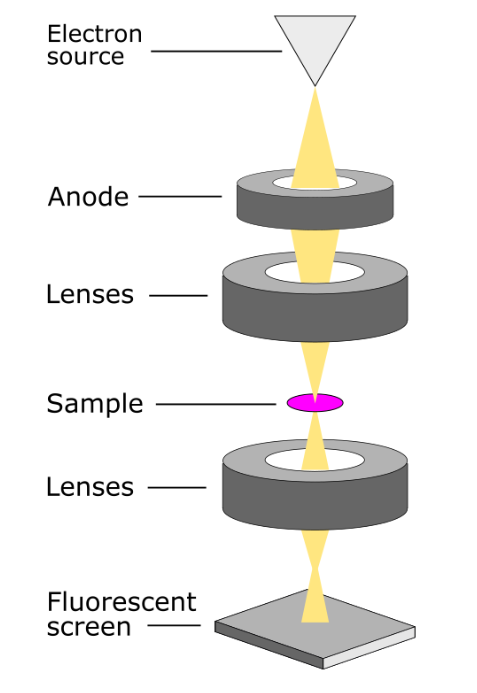
\includegraphics[width=0.45\textwidth]{img/TEM.png}
    \caption{Schematic diagram of Transmission Electron Microscope}\label{fig:TEM Schematic diagram}
    \tiny Source: \url{https://anapath.ch/electron-microscopy-2/}
\end{figure}

\vspace{20pt}

Additional lenses concentrate the transmitted electrons so they may be captured as an image on a detector or camera \cite{Gault2008}. The transmission electron microscope (TEM) may provide magnifications of up to 2 million times \cite{Gault2008}, which enables the viewing of structures and details on a scale as tiny as a nanometer or an angstrom. Because of this, it is an extremely useful instrument for study in materials science, cell biology, molecular structure analysis, and semiconductors \cite{Gault2008}. Imaging mode and diffraction mode are the major modes of operation for the transmission electron microscope (TEM) \cite{Adrian1984}. The image that is created by the transmitted electrons is used by the imaging mode. It is possible to examine either the diffraction pattern or the image depending on how the magnetic lenses are adjusted. The electron diffraction patterns are the primary focus of the diffraction mode, which focuses on the crystal structure \cite{Adrian1984}. The preparation of samples is an essential part of TEM. To facilitate electron transmission, specimens must have a thickness of between 50 and 100 nanometers (nm)\cite{Adrian1984}. Staining with substantial amounts of heavy metal salts is required for biological and polymer materials to produce contrast. Imaging of hydrated materials is possible because of specialized methods such as cryo-TEM, which vitrifies the samples \cite{Adrian1984}.

\vspace{10pt}

\begin{figure}[thbp]
    \centering
    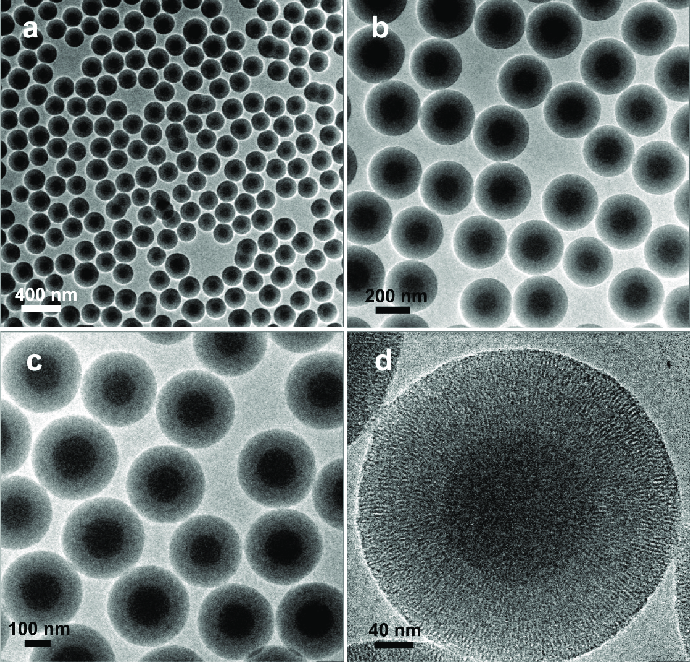
\includegraphics[width=0.5\textwidth]{img/TEM_MCM-41.png}
    \caption{TEM images of a mesoporous material(MCM-41) at different magnifications \cite{Loiseau2019}}\label{fig:TEM images of a mesoporous material}
    % \tiny Source: \url{https://pubmed.ncbi.nlm.nih.gov/31185689/}
\end{figure}


There is a possibility that radiation will destroy sensitive specimens, which is one of the TEM's limitations \cite{Egerton2004}. Imaging of living biological samples is likewise not possible due to the vacuum environment. Nevertheless, TEM continues to be an essential instrument for high-resolution structural characterization in both the physical and biological sciences \cite{Egerton2004}. In this study, transmission electron microscopy was used to examine Janus-like particles that were created from block copolymers. TEM gives the resolution and contrast necessary to clearly examine the nanostructure morphology and surface topology of the Janus particles \cite{Tang2017}.


\subsection{Neural 3D shape representations}
Major innovations in deep learning have enabled neural networks to automatically represent and render complex 3D shapes \ref{fig:DeepSDF's 3D bunny shape representation}, which was not previously feasible \cite{Park2019}. Neural implicit models can effectively represent shapes by mapping 3D coordinates to occupancy probabilities, signed distance values, or view-dependent radiance \cite{Mescheder2018}. This contrasts with traditional explicit surface and volumetric representations like meshes and voxels.

\vspace{10pt}

Early works focused on learning continuous signed distance functions for representing 3D surfaces on synthetic shape datasets \cite{Sitzmann2020}. Subsequent techniques aimed to relax the dependence on 3D supervision by formulating differentiable rendering losses that could be optimized using only 2D images \cite{Wu2015}. However, these approaches were limited to simplistic and smooth shapes.
\vspace{10pt}

\begin{figure}[thbp]
    \centering
    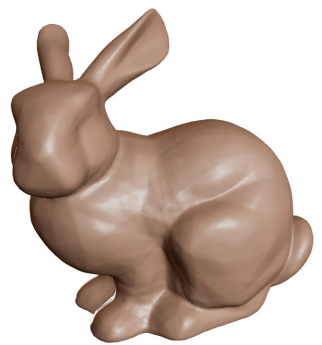
\includegraphics[width=0.5\textwidth]{img/Neural 3D representation.png}
    \caption{DeepSDF's 3D bunny shape representation \cite{Park2019}}\label{fig:DeepSDF's 3D bunny shape representation}
\end{figure}

More recently, coordinate-based neural radiance fields have achieved significant improvements in modeling complex real-world 3D scenes \cite{Mildenhall2020}. Novel photorealistic views of complex scenes can be created by expressing scene attributes such as volume density and view-dependent emitted radiance as continuous 5D functions.

\vspace{10pt}

In this work, we investigate leveraging the capabilities of modern neural 3D representations to reconstruct and denoise volumes from transmission electron microscopy tilt series. By training these networks to map from noisy TEM observations to cleaner target volumes in a self-supervised manner, they may learn specialized priors relevant to electron microscopy. Coordinate-based modeling may also better capture critical local context compared to other 3D approaches. This could significantly enhance the interpretability of fine structural details from TEM tomograms.


\subsection{Novel view Synthesis}
The act of creating fresh photographic perspectives on a subject from one or more input photos is called \textbf{View synthesis}  \ref{fig:Multi-view to Novel view synthesis}. This may be done with either a single image or many images. This allows the create unique synthetic viewpoints using only a small amount of photographic data. View synthesis is useful in a variety of contexts, including virtual reality, augmented reality, and the reconstruction of three-dimensional models\cite{Xia}.
Many different techniques have been used for view synthesis. The multi-view stereo approach builds a three-dimensional reconstruction of a scene by piecing together a few photographs obtained with a variety of cameras \cite{Seitz2006}\cite{Xia}. Then, this model may be displayed from any perspective.     Image-based rendering distorts and interpolates pixels depending on the original inputs to infer new viewpoints \cite{Chen2023}. These methods concentrate on identifying correspondences between different pictures.
\vspace{10pt}
\begin{figure}[thbp]
    \centering
    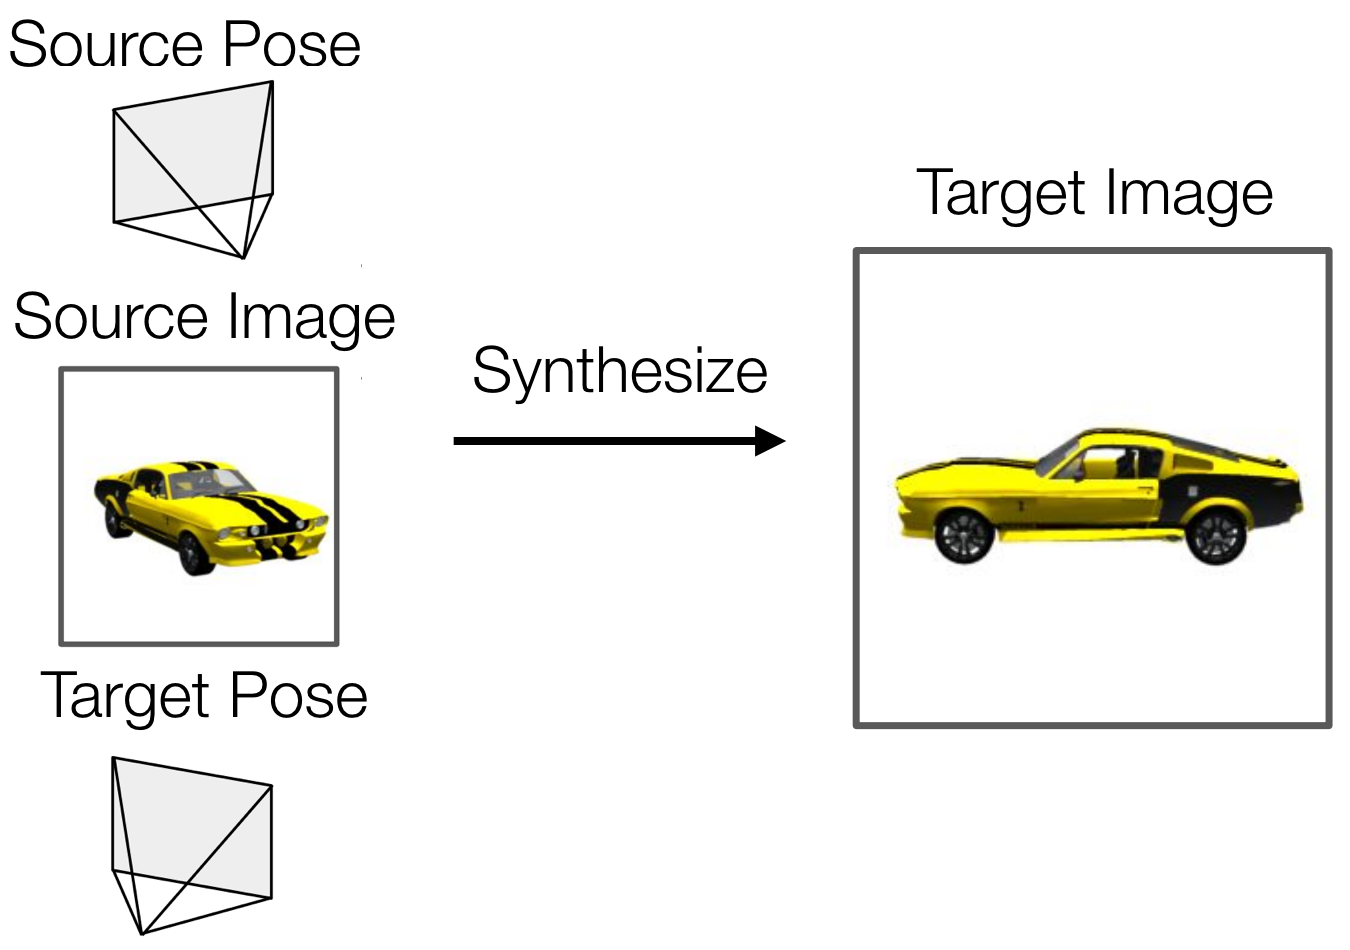
\includegraphics[width=0.6\textwidth]{img/novel view}
    \caption{Multi-view to Novel view synthesis\cite{Hartley2000}}\label{fig:Multi-view to Novel view synthesis}
\end{figure}

The most recent deep learning algorithms develop an implicit representation of the image generation process using neural networks. The neural rendering algorithms directly produce unique views by making predictions about the values of pixels based on the attributes of the scene that they have learned. Neural radiance fields (NeRF) \cite{Mildenhall2020} is a method for efficiently encoding a scene as a continuous five-dimensional function that maps three-dimensional coordinates to volume density and view-dependent brightness\cite{Mildenhall2020}. The continuous volumetric scene representation that NeRF provides has made it possible to do photorealistic view synthesis with only a few photos.
\vspace{10pt}
The capacity to implicitly infer a three-dimensional structure and appearance from just two-dimensional supervision is the primary benefit offered by neural view synthesis systems. Because of this, formal three-dimensional modeling or estimate is not required. These learning-based systems continue to increase the realism and flexibility of new view creation across a wide variety of applications, including augmented reality, virtual tourism, and 3D photography \cite{Fang}.
\clearpage
\subsection{Camera Parameters}
The geometric and optical properties of a camera are referred to as its camera parameters. These parameters define how a camera constructs a picture from the 3D world \cite{Hartley2000}. Understanding the process of picture generation as well as the tasks involved in 3D computer vision, relies heavily on an accurate representation of these factors.


\vspace{20pt}

\begin{figure}[thbp]
\centering
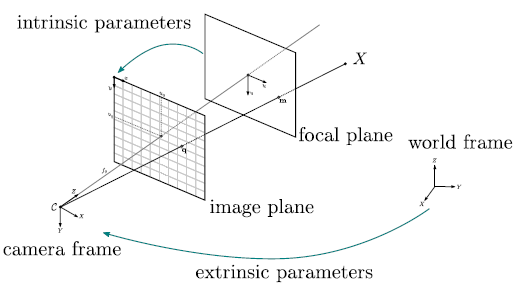
\includegraphics[width=.7\textwidth]{img/Camera.png}
\caption[Schematic Representation of Camera Parameters]{Schematic Representation of Camera Parameters. Source: \href{https://openmvg.readthedocs.io/en/latest/openMVG/cameras/cameras/}{OpenMVG Documentation}.}\label{fig:camera-parameters}
\end{figure}



\vspace{10pt}

\textbf{Intrinsic Parameters} are those that are unique to a camera and are not affected by the scene \ref{fig:camera-parameters}:
\begin{itemize}
  \item \textbf{Focal Length ($f$)}: The distance from the optical center to the image plane when the image is sharp. A primary component that determines both the field of view and the magnification \cite{Heikkila1997}. When dealing with non-square pixels, the x and y axes may have unique values.
  \item \textbf{Principal Point ($c_x, c_y$)}: The coordinates $(c_x, c_y)$ of the image center on the sensor plane. It accounts for lenses that are not perfectly aligned \cite{Heikkila1997}.
  \item \textbf{Skew Coefficient ($\alpha$)}: A rotation of the axis between the pixel grid and the sensor that considers non-rectangular pixel shapes \cite{Heikkila1997}. Produces a shearing transformation when applied.
  \item \textbf{Distortion Coefficients}: This model simulates optical distortions such as radial, tangential, and narrow prism effects. Radial is the most noticeable and gives an impression like a barrel or pincushion \cite{Heikkila1997}.
\end{itemize}

The intrinsic camera matrix $K$ can be represented as:

\begin{equation}
K = \begin{bmatrix}
f_x & \alpha & c_x \\
0 & f_y & c_y \\
0 & 0 & 1
\end{bmatrix}
\end{equation}

where $f_x$ and $f_y$ are the focal lengths expressed in pixel units.

\vspace{30pt}

\textbf{Extrinsic Parameters} are determined by the position of the camera in relation to the world \ref{fig:camera-parameters}:
\begin{itemize}
  \item \textbf{Rotation Matrix ($R$)}: A 3x3 matrix describing the camera's orientation in a world coordinate system \cite{Zhang2000}. Represented by a sequence of rotations (Euler angles).
  \item \textbf{Translation Vector ($\mathbf{T}$)}: A vector defining the position of the camera's origin in world coordinates \cite{Zhang2000}.
\end{itemize}

The extrinsic parameters are combined into a 3x4 matrix [$R$ | $\mathbf{T}$], defining the transformation from world coordinates to camera coordinates.

\vspace{10pt}

Together, intrinsic and extrinsic parameters form the camera projection matrix $P$, which is responsible for mapping 3D world points into 2D picture coordinates:

\begin{equation}
P = K \times [R | \mathbf{T}]
\end{equation}

For computer vision applications like posture estimation, 3D reconstruction, and unique view synthesis, accurate assessment of these parameters is essential.


\vspace{10pt}

Applications in augmented reality \cite{Zhang1995}, autonomous navigation \cite{Zhang1995}, and computational photography \cite{Zhang1995} heavily rely on precise camera calibration. Adapting camera models to new modalities, such as light field imaging, continues to be an active area of research.


\subsection{COLMAP}

COLMAP is an open-source pipeline that uses structure-from-motion (SfM) and multi-view stereo (MVS) to generate 3D models from 2D images \cite{Schönberger}. Through solid correspondence construction, global optimization, and volumetric fusion, it features state-of-the-art reconstructions.

\begin{itemize}
  \item \textbf{Feature Extraction and Matching}

    First, appearance-based image features that can be paired between views are found and described \ref{fig:COLMAP camera position extracting from 2D images}. Based on local gradients, SIFT is frequently used to locate scale- and rotation-invariant key points \cite{Lowe1999}. Each key point has a high-dimensional descriptor vector that is insensitive to noise, perspective, and illumination \cite{Lowe1999}.
    \vspace{10pt}
      Based on similarity measures like Euclidean or cosine distance, an effective closest neighbor search matched characteristics between image pairings. Uncertain matches can be eliminated with the ratio test \cite{Lowe1999}. Outlier matches that are inconsistent with a single 3D point are eliminated by geometric verification using RANSAC \cite{Lowe2004}.

    \begin{figure}[thbp]
    \centering
    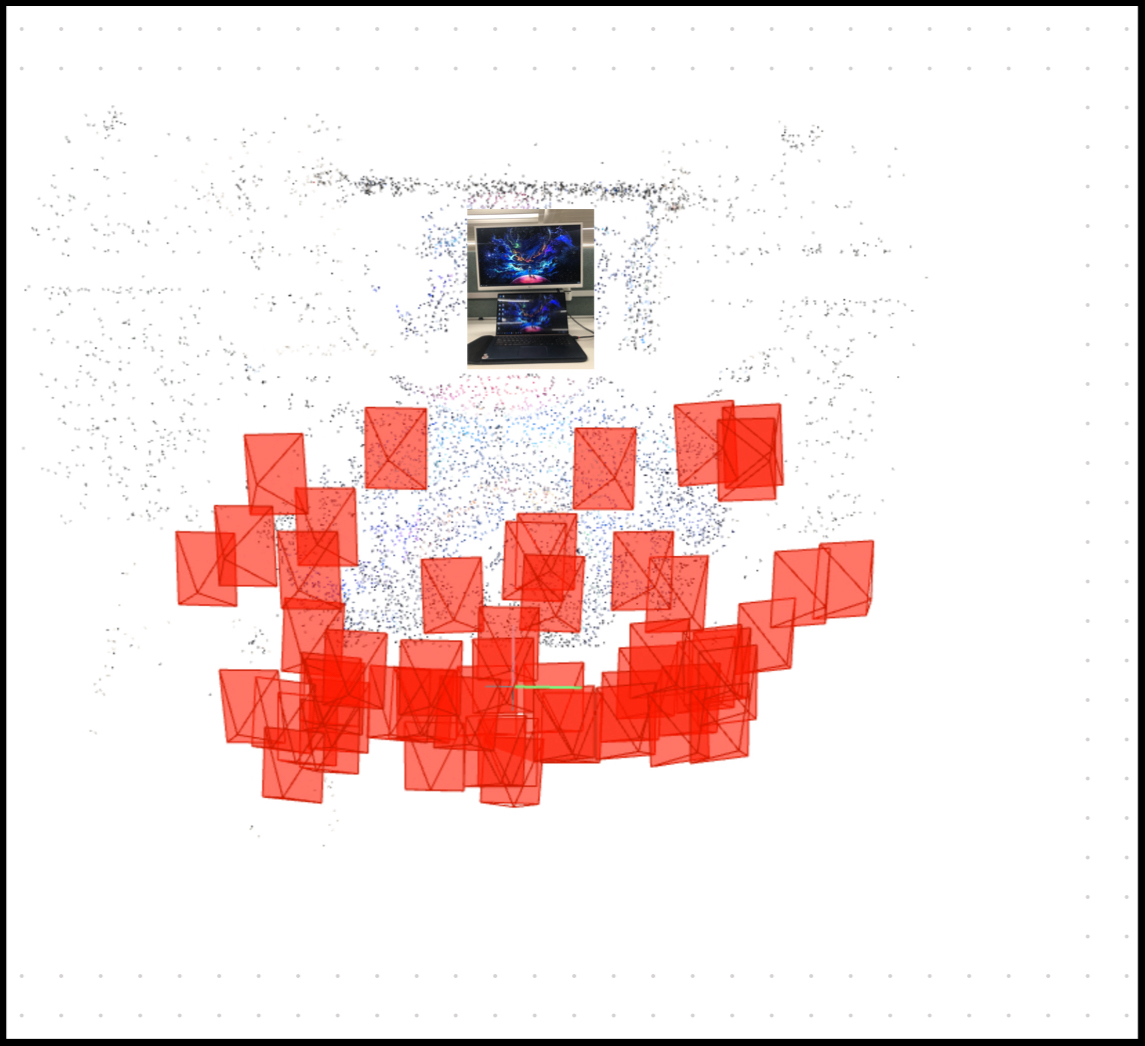
\includegraphics[width=0.6\textwidth]{img/Colmap.png}
    \caption{COLMAP camera position extracting from set of 2D images}\label{fig:COLMAP camera position extracting from 2D images}
    \end{figure}

  \item \textbf{Incremental Structure from Motion (SfM)}
    
     In an incremental SfM method, the registered 2D-2D matches create initial sparse 3D point clouds \cite{Fischler1981}. An initial point cloud is plotted using an initial image pair. Which views to update next are efficiently chosen by robust visibility constraints \cite{Fischler1981}. With points recursively mapped from fresh views \cite{Snavely}, camera poses are predicted using a Straight Linear Transform within a RANSAC cycle.
    
  \item \textbf{Global SfM Optimization}
    
     Utilizing bundle adjustment, the progressive reconstruction is globally improved to improve camera simultaneously poses and 3D point coordinates. Scale drift is reduced with regularization. Bundle adjustment reduces the top view error between the positions of anticipated and actual 2D features in all perspectives \cite{Heinly}. This enhances accuracy and comprehensiveness.
    
  \item \textbf{Multi-View Stereo (MVS) Depth Map Estimation}
    
     The optimal cameras and points start the estimate of the multi-view stereo depth map. Using photo consistency metrics such as normalized cross correlation between distorted picture patches, dense correspondence is created in each view \cite{Triggs}. Accuracy is improved by regularization using filtering such as Gaussian smoothing \cite{Galliani}. The per-view depth maps that are constructed include geometric detail.
    
  \item \textbf{Surface Reconstruction}
    
      When creating a final 3D surface mesh, volumetric fusion methods such as screening Poisson reconstruction are utilized to merge the depth data to produce the mesh \cite{Facciolo2015}. It accomplishes this by interpolating an indicator function to provide a continuous and smooth surface. Additional post-processing steps, such as graph cuts-based optimization \cite{Kazhdan}, may be utilized to improve details even further. Realism and color are added when texturing with the use of input images.
     
  
\end{itemize}

\clearpage
\subsection{NeRF (Neural Radiance Field)}

Neural radiance fields (NeRF) are a recent breakthrough technique for novel view synthesis and 3D scene modeling using implicit neural representations \cite{Mildenhall2020}. NeRF represents a scene as a continuous 5D radiance field (3D position + 2D viewing direction) using a multilayer perceptron (MLP).
\vspace{10pt}

\begin{figure}[thbp]
\centering
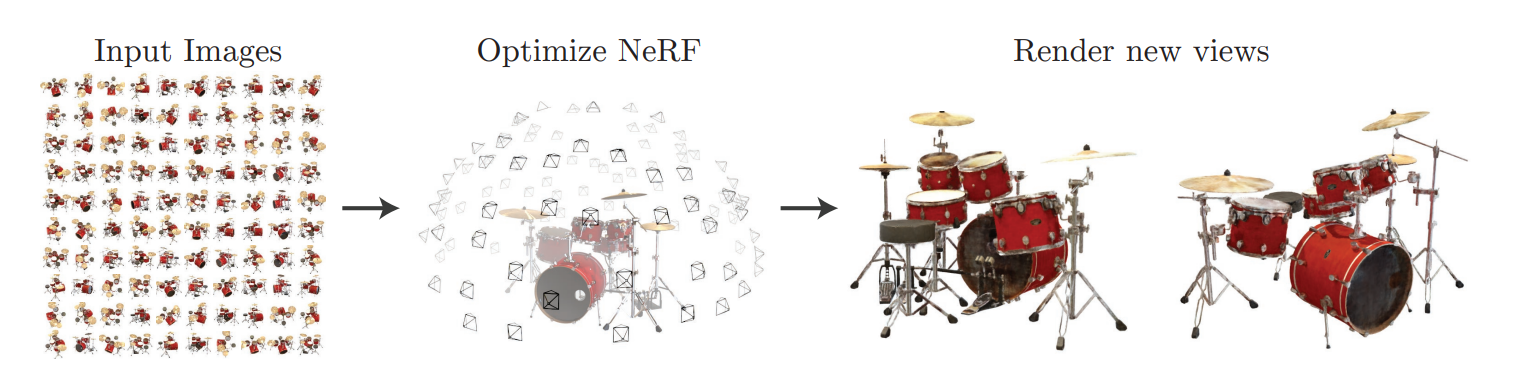
\includegraphics[width=1\textwidth]{img/NERF.png}
\caption{Conceptual Illustration of Neural Radiance Fields (NeRF) \cite{Mildenhall2020}}\label{fig:Conceptual Illustration of Neural Radiance Fields (NeRF)}
\end{figure}

\vspace{10pt}

\begin{algorithm}
\caption{Training Neural Radiance Field (NeRF)}
\begin{algorithmic}[1]
\STATE Initialize MLP with random weights.
\FOR{each training iteration}
    \STATE Select a subset of input images.
    \FOR{each selected image}
        \STATE Sample a set of rays passing through image pixels.
        \FOR{each ray}
            \STATE Sample points along the ray.
            \STATE Query MLP for color and density at each point.
            \STATE Calculate the rendered color of the ray using volume rendering.
        \ENDFOR
        \STATE Calculate loss between rendered and actual pixel colors.
        \STATE Update MLP weights to minimize the loss.
    \ENDFOR
\ENDFOR
\end{algorithmic}
\end{algorithm}
\vspace{10pt}

    
The MLP maps each (x,y,z) location in space to an RGB color value and volume density scalar. The color indicates the emitted radiance, while density encodes occlusion. Querying this MLP at sampled points along camera rays enables volumetric ray marching to render novel views. The integral of density * color approximates the total radiance along each ray.
Compared to discrete voxel grids or meshes, continuous coordinate-based modeling better captures smooth variations in structure, appearance, and lighting. The MLP can represent complex scenes in a memory-efficient compact latent code rather than an explicit 3D model. Adjusting MLP weights based on rendered and real image differences allows for optimizing the scene representation.
\vspace{10pt}

\clearpage
Key advantages of the NeRF approach include:
\begin{itemize}
 \item Coordinate MLPs effectively model local relationships.
 \item Continuous representation enables high-quality view interpolation.
 \item Volume density handles complex occlusion effects.
 \item View-direction encoding models view-dependent phenomena like highlights.
\end{itemize}
\vspace{10pt}



    
NeRF obtains impressive results in reconstructing 3D scenes from only a sparse set of input views (e.g. 20-50 images). However, it relies on accurate camera pose estimation and clean photographic inputs. The utility for noisy domains like biomedical imaging is still being explored. For training purposes, you will need the camera parameters for the images that have been provided. These camera parameters are typically computed by SfM tools like COLMAP \cite{Mildenhall2020}.


\vspace{10pt}


\subsubsection{Self-Supervised Learning in NeRF for TEM Data}

Self-supervised learning, a robust approach for training neural networks in the absence of labeled data, leverages the intrinsic structure of data to guide representation learning, especially in fields where manual annotations are scarce \cite{Kolesnikov2019}. In our work, we explore this paradigm in the context of TEM data, focusing on a self-supervised framework specifically designed for neural radiance fields (NeRF) to address unique challenges in TEM imaging.

\vspace{10pt}

NeRF models are typically trained with posed 2D image datasets and associated camera parameters, utilizing view reconstruction losses for supervision \cite{Mildenhall2020}. However, in TEM, obtaining accurate poses is challenging due to issues like low signal-to-noise ratios and incomplete angular coverage, rendering standard structure-from-motion techniques ineffective. Our approach overcomes these hurdles by leveraging principles of geometry \cite{Chiyu2020} and appearance consistency \cite{Chiyu2020}, replacing traditional supervision methods with self-supervision that relies on the geometric and appearance consistencies across input views.

\vspace{10pt}
In our proposed method, NeRF synthesizes target images from a TEM tilt series using a subset of the images, thus inferring a consistent 3D representation. The process involves random sampling of training directions, predicting images along held-out directions through volumetric raymarching, and using the MLP scene representation. The reconstruction loss between predicted and actual images serves as self-supervision for the model, enabling it to learn to predict complete volumes from sparse, noisy data. This method allows NeRF to implicitly learn priors suitable for electron tomography. Our experiments show that this self-supervised, coordinate-based approach effectively reconstructs higher fidelity volumes from limited input compared to other methods, highlighting its potential to address key computational challenges in TEM analysis \cite{Sitzmann2020}.


\clearpage
\subsection{Enhanced Super-Resolution Generative Adversarial Networks (ESRGAN)}

An overview of Enhanced Super-Resolution Generative Adversarial Networks (ESRGAN) \cite{Xintao2018} shows that this technology is a major step forward in the super-resolution of images \ref{fig:ESRGAN Architecture} This deep learning model is an essential tool in industries that need high-resolution imaging because it is made to boost image resolution beyond what the sensor can handle. ESRGAN is a development of the previous Super-Resolution GAN (SRGAN) \cite{Ledig2017}, but it has undergone significant improvements that enable it to produce images with finer features and more realistic textures \cite{Blau2018}.



\begin{figure}[thbp]
\centering
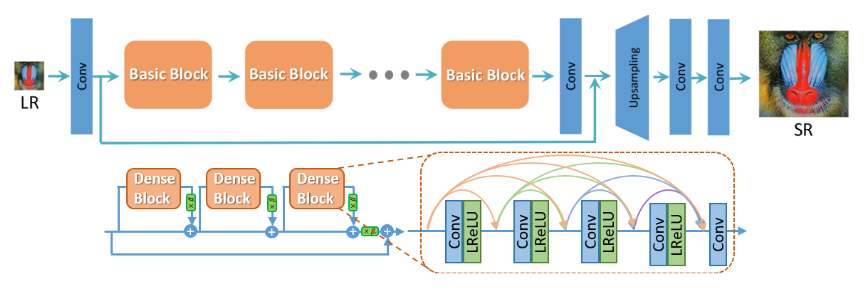
\includegraphics[width=1\textwidth]{img/ESRGAN.png}
\caption{ESRGAN Architecture \cite{Xintao2018}}\label{fig:ESRGAN Architecture}
\end{figure}



The implementation of Residual-in-Residual Dense Blocks (RRDB) to enhance the model's depth and parameters and make optimization simpler is one of ESRGAN's primary advantages over SRGAN. Additionally, it introduces the Relativistic GAN (RaGAN) loss, which helps to improve texture details and sharpen edges. Furthermore, ESRGAN uses a perceptual loss that makes use of pre-trained features from VGG networks, which improves the super-resolved images' perceived quality \cite{Xintao2018}.

\vspace{10pt}
Especially useful in TEM context, ESRGAN may infer high-resolution images four times larger than the input \cite{Xintao2018}. The more realistic textures of the model are essential for improving medical images and computational microscopy. The ability of ESRGAN to synthesize fine details is utilized as a post-processing step for processed TEM data in our thesis study. This application is essential in order to improve the quality of TEM images, where the clarity of microscopic structures and details is crucial.

\vspace{10pt}
Our thesis tackles the problem of enhancing the resolution and perceived quality of TEM pictures through the implementation of ESRGAN. Our goal in using ESRGAN is to improve these images' diagnostic utility and aesthetic appeal so that they may be used for more in-depth examination and interpretation. One example of how cutting-edge deep learning techniques are being used in practice to improve scientific imaging is the incorporation of ESRGAN into the pipeline for processing TEM pictures. This method advances the science of microscopy while also establishing a standard for the use of super-resolution techniques in other fields where improved picture quality and resolution are necessary.